\graphicspath{{chapters/images/07/}}
\chapter{16S-rRNA sequencing}

\section{Introduction to metagenomics}

  \subsection{Definition of metagenomics}
   The term metagenomics refers to the study of uncultured microorganisms from the environment, which can include humans or other living hosts with focus on taxonomic and functional characteristics of the total collection of microorganisms within a community.
   The main way to analyse the entire microbial population of an environment is through high-throughput sequencing of nucleic acids isolated from the sample.
   Two approaches can be distinguished:

   \begin{multicols}{2}
     \begin{itemize}
       \item 16S rRNA gene sequencing.
         \item Shotgun metagenomic.
     \end{itemize}
   \end{multicols}

  \subsection{Why studying the metagenome}
   Microbes are basically everywhere, in and outside of our bodies, in oceans, glaciers, hot springs and rocks.
   Given how widespread and abundant microbes are, studying the metagenome provides us plenty of information both on human and non-human microbiome and environment.
   For instance, it has been shown that the microbiome correlates to several diseases, therefore it can be used as a non-invasive biomarker.
   The list of activities microbes are involved in is constantly increasing.

  \subsection{Differences with older microbiome studies}
  The microbiome was discovered many years ago but there were no tools to analyze it properly: the only way was to culture and isolate each bacterium.
  This is an unfeasible approach to study the entire community, since only some bacteria can be grown in the laboratory and it would take an unreasonably long amount of time.
  The advent of high-throughput technologies is what made possible to study the microbiome of a sample, reducing significantly times, costs and increasing substantially the fraction of the microbiome that can be known.

  \subsection{Example: skin microbiome}
  Some studies were performed on skin microbiome (Segata et al, Nature Methods 2012, Truong et al, Nature Methods, 2015).
  Only about $60\%$ of the contigs of various size were mapped to known microbes while $40\%$ belonged to unknown species.
  When separating these sequences based on GC content and abundance, many clusters formed, some with higher abundance while others with lower abundance, probably due to the low GC content that makes more difficult for the machine to sequence them, therefore causing them to be underestimated.
  Studying this $40\%$ of unknown sequences is one of the main tasks of metagenomics.

\section{16S rRNA sequencing}
16S rRNA sequencing is one of the first techniques developed to study the microbiome, since it does not require a huge amount of sequences nor excessive costs.

  \subsection{Simplified 16S rRNA analysis workflow}
    The general workflow for a 16S rRNA analysis is the following:

    \begin{multicols}{2}
      \begin{itemize}
        \item DNA extraction from the entire community present in the sample.
          Some bacteria will be over-represented while other will be under-represented.
        \item Selective PCR amplification of 16S rRNA gene.
        \item High-throughput sequencing.
        \item Sequence mapping against genomes in databases.
          This allows to define which bacteria and which variants of those are present in the sample and to find new and unknown bacteria.
      \end{itemize}
    \end{multicols}

    \begin{figure}[H]
      \centering
      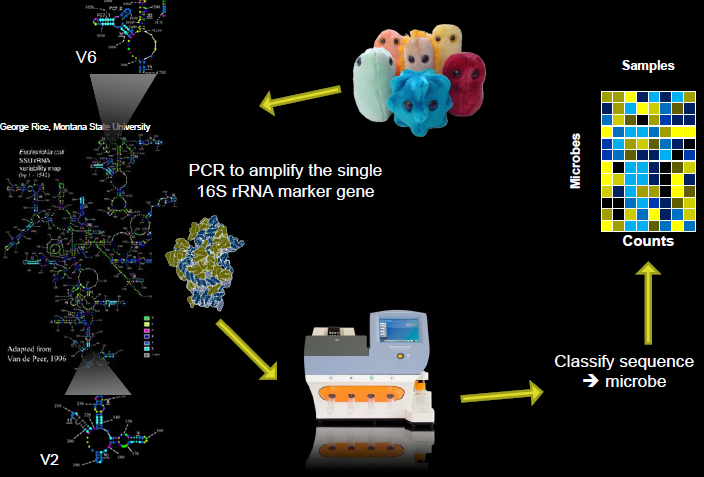
\includegraphics[width=0.9\textwidth]{general_workflow.png}
      \caption{\label{fig:general_workflow}General 16S gene analysis workflow}
    \end{figure}

  \subsection{16S rRNA gene}
    The ribosome is one of the most conserved, if not the most conserved, structure in all living organisms, making it one of the best phylogenetic markers.
    In prokaryotes, the ribosome is composed of several elements, both proteic and RNA based.
    Of the RNA based ones, $3$ of them are ribosomial RNAs (rRNAs), namely 5S, 16S, 23S.
    Since these components are fundamental for any bacterium, all bacteria present the genes codifying for these rRNAs.
    Moreover most of the sequences are highly conserved but some regions have some species-specific variability which can be used as a barcode to find and classify species.
    The most conserved of the rRNAs is 23S but the one used for microbiome analysis is 16S (which corresponds to the human 18S).
    Its gene is a few thousands nucleotides long, most of which are highly conserved.
    The bulk of the differences among species is in the hypervariable regions named V1 to V9, the terminal loops of the structure.
    They are regions far away from the catalityc site.
    Despite the high degree of conservation, some variability can be found outside the hypervariable regions too.
    The annotation of which portions of the 16S rRNA gene are conserved has been performed using E. coli as a reference.
    For a few hundred organisms the gene has been compared to the reference one to define the degree of conservation of each stretch of nucleotides.
    Some totally conserved regions  are present but they are not very big.

    \begin{figure}[H]
      \centering
      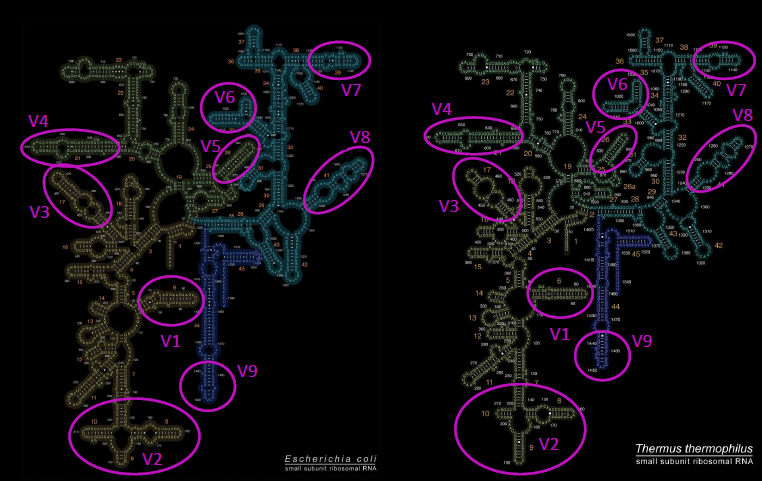
\includegraphics[width=0.9\textwidth]{16S_rRNA.png}
      \caption{\label{fig:16S_rRNA}Structure of the 16S rRNA in \textit{E. coli} and \textit{T. termophilus}}
    \end{figure}

  \subsection{Primer and high-throughput machine choice}
    One could sequence the entirety of the 16S rRNA gene, for example using NanoPore seq, but this would introduce many errors that could lead to mapping the sequence to the wrong organism.
    For this reason it is preferred to amplify only certain specific regions of the gene.
    To study the microbiome in a high-throughput way primers which can bind to all species are needed.
    Since the sequences conserved in all species are too short, you use primers that bind highly conserved regions.
    For this reason, regardless of which primers you choose there will be a bias in your results: some species will not be identifiable using those primers.
    This bias can be somewhat minimized using in silico primer validation, which means testing your primers against databases of 16S tRNA genes like silva and green genes, to test and decide the best pair of primers for your experiment.

    \begin{figure}[!h]
      \centering
      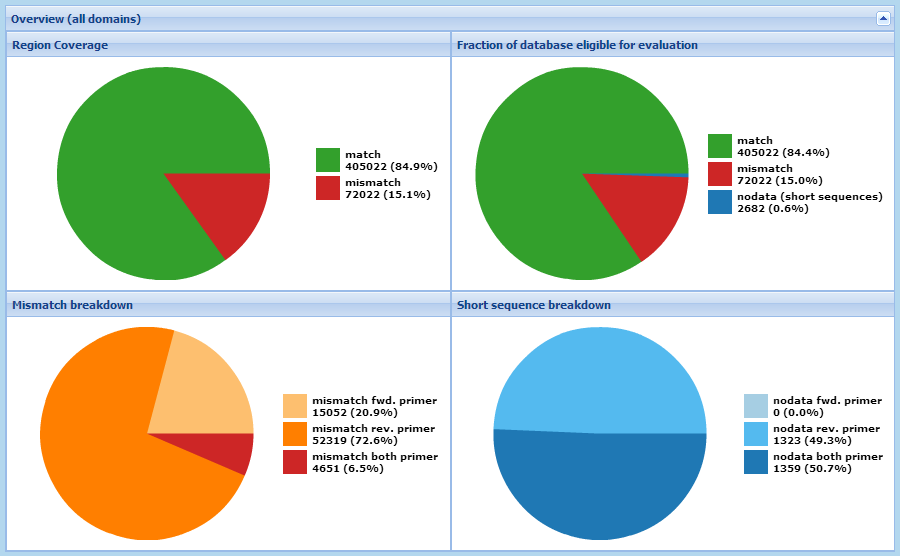
\includegraphics[width=0.9\textwidth]{silva_analysis.png}
      \caption{\label{fig:silva_analysis}Example of \textit{in silico} primer validation using silva; you can notice the different efficiency of the primers relative to different parameters.}
    \end{figure}

    Still, two experiments conducted with different primers will always have some differences.
    Moreover the binding regions must flank some variable region, in order to include it in the amplicon.
    Finally pair end amplification both primer back and forward is needed in order to have the complete amplicon to make the comparison easier.
    Given these characteristics there are multiple possible priming sites based on the sequence and on chemical properties of the primers.
    Moreover, primers can be used as forward or reverse to obtain different combinations and sequences.

    \begin{figure}[!h]
      \centering
      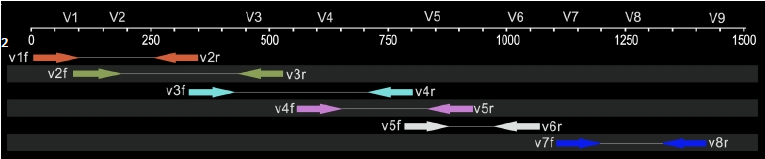
\includegraphics[width=0.9\textwidth]{primer_placement.png}
      \caption{\label{fig:primer_placement}Examples of common primer placements relative to hypervariable regions}
    \end{figure}

    As an example of the importance of the choice of primers, in some skin microbiome analyses, researchers could not find two bacteria always present on human skin due to the choice of primers.
    Moreover S. aureus seemed over-represented due to the non-amplification of other important species.
    Despite the biases, this technique is still extremely useful.

    There are different protocols to target conserved regions also based on the machine used.
    In general:

    \begin{multicols}{2}
      \begin{itemize}
        \item Sanger machines are not very good for this application since they have low throughput and they are more suited for longer sequencing tasks.
        \item Roche 454 machines have historically been well suited, since it was possible to sequence three hypervariable regions together using $400$ nucleotides reads, providing a good cost and throughput trade-off.
        \item Illumina HiSeq is not the optimal choice since it has shorter reads and unnecessarily high throughput.
          Illumina MiSeq and IonTorrent can be a decent compromise.
      \end{itemize}
    \end{multicols}

  \subsection{In depth 16S rRNA analysis workflow}
  Adding detail, a more complete overview of the 16S rRNA analysis workflow is:

  \begin{multicols}{2}
    \begin{itemize}
      \item DNA extraction from each of your samples
      \item Selective PCR amplification of 16S rRNA gene, introducing a barcode in the sequences using tagged primers.
      \item High-throughput sequencing of all the samples in a single run to reduce costs.
        The result is a set of amplicons belonging to different samples and with a barcode attached.
      \item Demultiplexing, which means removing the barcodes and assigning each sequence  to the corresponding sample.
        Sequencing noise must be taken into account, therefore low quality reads must be removed.
      \item Multiple sequence alignment against reference sequences.
        Some reads will probably not map to any reference sequence.
      \item Group related sequences into OTUs (operational taxonomic units), which means grouping sequences that share some common variants.
        Since SNPs in the microbial genome are present, the similarity threshold between sequences cannot be too restrictive.
        OTUs can be used to define the relative abundance of each species in the sample, but in order to do so it is necessary to normalize for the copy number of the 16S gene sequence.
        This is very difficult since an accurate estimate can be made only if long read sequencing has been performed on the organism, which is almost never the case since for microbes that basically corresponds to full genome mapping.
      \item Build phylogenetic tree using one representative for each OTU.
      \item Annotate the OTUs using 16S gene databases.
      \item Downstream analysis is performed, such as clustering to visualize similarities among samples.
    \end{itemize}
  \end{multicols}

    \begin{figure}[!h]
      \centering
      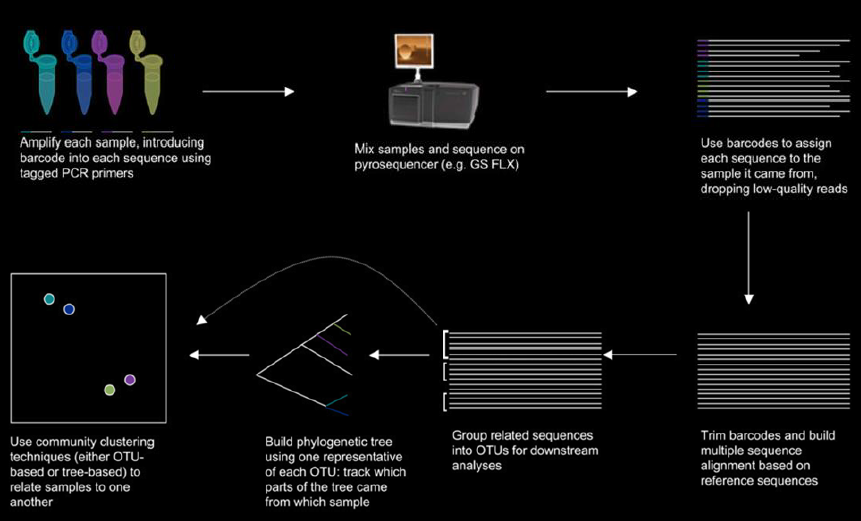
\includegraphics[width=0.9\textwidth]{expanded_workflow.png}
      \caption{\label{fig:expanded_workflow}Expanded 16S gene analysis workflow}
    \end{figure}

    \begin{figure}[!h]
      \centering
      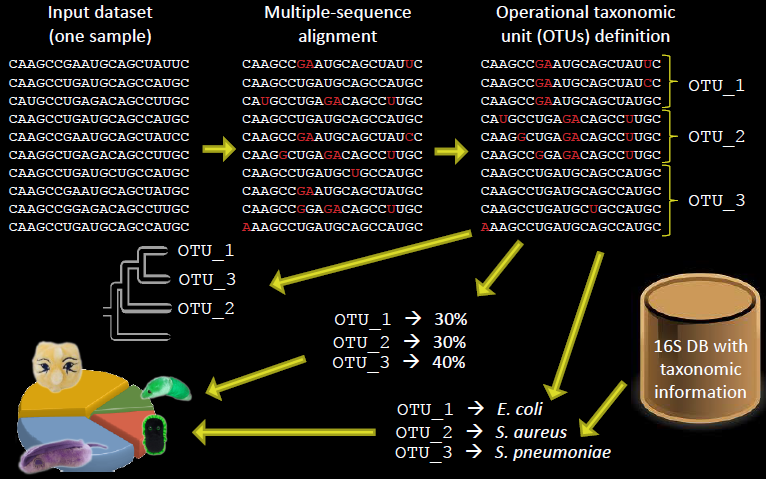
\includegraphics[width=0.9\textwidth]{zoom_in_16S.png}
      \caption{\label{fig:zoom_in_16S}Zoom in on 16S gene analysis workflow}
    \end{figure}

  \subsection{OTU clustering}
  Defining OTUs requires using multiple sequence alignment.
  Since this approach is a generalization of the mapping algorithm it is quite complex in terms of speed, but still feasible.
  Generally greedy algorithms which add the lowest possible amount of gaps are used to perform multiple sequence alignment.
  After the alignment, sequences are split into OTUs (operational taxonomic units), which are groups of 16S sequences very similar to each other.
  Generally a sequence is defined as the representative of the OTU, meaning that it has a certain threshold of identity with all other sequences in the OTU, usually $97\%$ when considering species and that minimizes the differences of all other sequences of the OTU with itself.
  Some OTUs can be assigned univocally to a species, some others may be associated to more species, some others cannot be mapped to know species.
  The fact that a species may map to multiple OTUs is often an error but it may sometimes allow to find subspecies.

    \begin{figure}[!h]
      \centering
      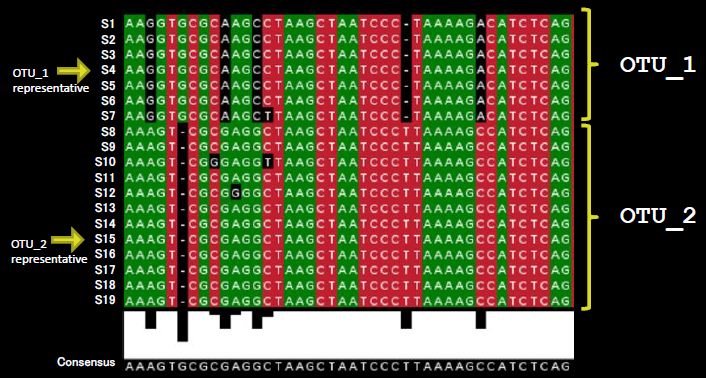
\includegraphics[width=0.9\textwidth]{OTU_general.png}
      \caption{\label{fig:OTU_general}Example of multiple sequence alignment for OTUs}
    \end{figure}

    After sequence alignment, OTU clustering can be done through several supervised or unsupervised learning methods.
    The most common unsupervised clustering methods are:

    \begin{multicols}{2}
      \begin{itemize}
        \item Single linkage clustering nearest neighbour: assign the sequence to a cluster if that OTU already contains at least a sequence similar enough ($97\%$).
          However two distant sequences in the OTU network could share a similarity which is way lower than $97\%$.
          This could result in underclustering.
        \item Complete linkage clustering furthest neighbour: assign the sequence to a cluster only if all the sequences of the OTU are similar enough ($97\%$).
          However two sequences may be similar enough, yet belong to different OTUs, because the overall cluster width, or divergence, is at most $3\%$.
          This approach could then generate different solutions, based on the order the points are added in.
          Moreover, if the clustering conditions are too stringent, sequencing errors and SNPs in the microbial genome may result in overclustering (defining too many clusters).
      \end{itemize}
    \end{multicols}

    \begin{figure}[!h]
      \centering
      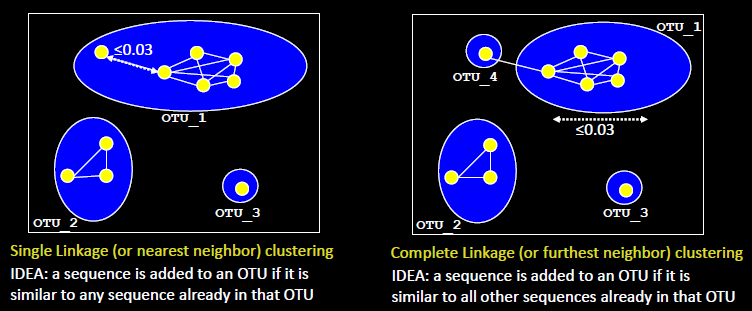
\includegraphics[width=0.9\textwidth]{clustering_methods.png}
      \caption{\label{fig:clustering_methods}Visualization of single linkage analysis and complete linkage analysis}
    \end{figure}

    \begin{figure}[!h]
      \centering
      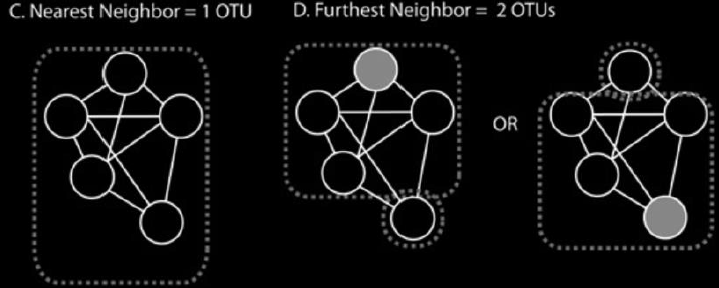
\includegraphics[width=0.9\textwidth]{overclustering.png}
      \caption{\label{fig:overclustering}Example of overclustering and result multiplicity due to complete linkage analysis}
    \end{figure}

  \subsection{OTU taxonomic annotation}
  Assigning a taxonomic annotation to an OTU cannot be done simply using BLAST to get the best matching sequence.
  This is because there is too much noise in the sequences and because it is difficult to classify new strains.
  A better way is using some other algorithm that assigns the terms of the taxonomic notation (since it is more than just one label) and provides some degree of confidence in the prediction.
  For instance the algorithm may be able to correctly assign the first taxonomical terms, up until Enterobacteriaceae, but then it provides a prediction of the OTU belonging to a list of species with confidence value for each one.

    \subsubsection{RDP classifier (Naive Bayes Model)}
    $P(S|G)$ is computed by RDP using a 8-mer strategy: comparing the 8-mers in $S$ with the 8-mers in all the training sequences available for genus $G$.
    The confidence of each prediction is computed by bootstrapping:

    \begin{multicols}{2}
      \begin{enumerate}
          \item Select a random subsequence of $S$, $S’$.
          \item Compute the $G$ that maximizes $P(S’|G)$.
          \item Repeat the procedure a number of times.
          \item The number of time $G$ is selected by the bootstrapping procedure is the confidence
      \end{enumerate}
    \end{multicols}

    Leave one-out-cross validation:

    \begin{multicols}{2}
      \begin{itemize}
          \item Take out one data point from the training set.
          \item Apply the classifier on the left-out point (without using it in the training set).
          \item Check the accuracy of the prediction.
          \item Repeat the procedure for each training data point.
      \end{itemize}
    \end{multicols}

    The RDP classification accuracy is evaluated with the leave-one-out cross validation on the training set of hundreds thousands of 16S references:

    \begin{multicols}{2}
      \begin{itemize}
          \item Accuracy is the percentage of correct classification (over the all leave-one-out runs).
          \item There are varying levels of taxonomic resolution (from phylum to genus).
          \item There are varying sequence lengths.
          \item In real applications accuracies are probably smaller due to sequencing errors or the presence of unknown bacteria.
      \end{itemize}
    \end{multicols}

\section{Diversity analysis}

\begin{figure}[h]
  \centering
  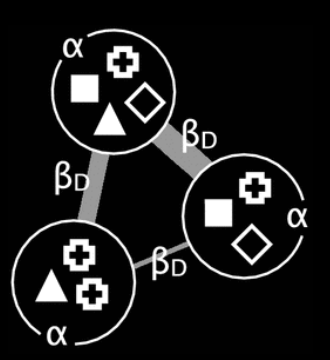
\includegraphics[width=0.6\textwidth]{Diversity.png}
  \caption{}
\end{figure}

  \subsection{Alpha diversity analysis}
  Alpha diversity analysis is a measure of how diverse or complex a microbial community is.
  It measures within sample diversity.
  Species richness is a widely use alpha diversity index.
  All individuals considered have non-zero abundance, some will have high abundance ($\sim99\%$) or low abundance ($1\%$).
  High alpha diversity are usually associated with populations that are more robust and resilient to changes.
  For examples gut microbiome with a high richness is usually associated with healthy state, instead of disease.
  Alpha diversity can be compared only between samples with the same sequencing depth.
  To do so between different samples usually a depth cut-off is chosen.

  \subsection{Beta diversity analysis}
  Beta diversity analysis is a measure of how different two microbial communities are.
  It measures between sample diversity.
  It is possible to measure the beta-diversity using the inverse of number of shared species.
  An example of beta-diversity is UniFrac.
  In UniFrac the distance is equal to the fraction of the total branch length that is unique to any particular environment.
  UniFrac can be also weighted in order to include abundances for each OTU.

  \begin{figure}[h]
    \centering
    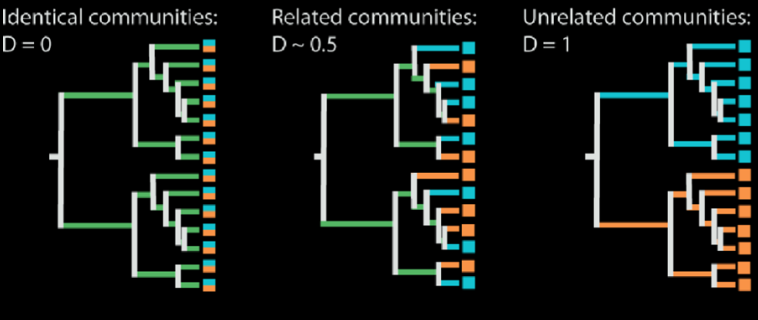
\includegraphics[width=0.6\textwidth]{UniFrac.png}
    \caption{\textbf{D=0.} Blue and orange samples always have the same OTUs. Each 16S (each branch) is present in both samples. \textbf{D=$\sim$0.5.}In reality we usually have a mix of the 2 situations. Some OTUs are present only in one of the samples and are either quite distant from the others or close (based on upstream the branch goes). \textbf{D=1.} Completely distinct OTUs . The difference is also in the upstream branches, which have different colors.}
  \end{figure}

  \subsection{Principal Coordinate Analysis}
  PCoA is also known as multidimensional scaling.
  It is one of the most powerful approaches for exploratory analysis.
  The idea is to represent the multidimensional relationship between samples in a two or three dimensional space.
  It is possible to use any similarity function as Euclidean distance, UniFrac, bray-Curtis distance.
  We find frequently hierarchical clustering plots.
  It is mostly done to visualize the similarities and difference between species, identifying for example cluster of species.
